% The roots of X^3-2 in C: one real embedding, one pair of complex embeddings (generated).
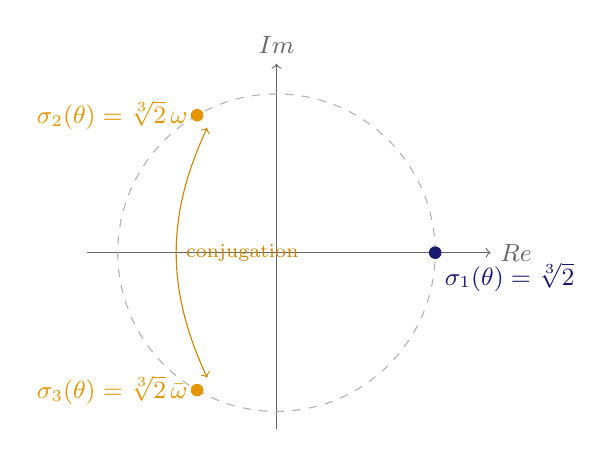
\begin{tikzpicture}[scale=1.6]
\draw[->,thin,black!60] (-1.5,0)--(1.7,0) node[right,font=\small]{$\operatorname{Re}$};
\draw[->,thin,black!60] (0,-1.4)--(0,1.5) node[above,font=\small]{$\operatorname{Im}$};
\draw[black!30,dashed] (0,0) circle (1.2599);
\fill[MidnightBlue] (1.2599,0.0000) circle (0.05) node[below right,font=\small]{$\sigma_1(\theta)=\sqrt[3]2$};
\fill[Orange!90!black] (-0.6300,1.0911) circle (0.05) node[left,font=\small]{$\sigma_2(\theta)=\sqrt[3]2\,\omega$};
\fill[Orange!90!black] (-0.6300,-1.0911) circle (0.05) node[left,font=\small]{$\sigma_3(\theta)=\sqrt[3]2\,\bar\omega$};
\draw[<->,Orange!80!black,thin] (-0.5500,0.9911) to[bend right=25] node[right,font=\scriptsize]{conjugation} (-0.5500,-0.9911);
\end{tikzpicture}
